\documentclass{article}
\usepackage{graphicx}
\usepackage{hyperref}
\usepackage{amsmath}

\usepackage{Sweave}
\begin{document}
\Sconcordance{concordance:sweave_example.tex:sweave_example.Rnw:%
1 5 1 1 0 14 1 1 2 7 0 1 2 4 1 1 2 7 0 1 2 4 1 1 4 3 0 4 1 3 0 1 2 2 1 %
1 2 23 0 1 2 4 1 1 3 2 0 2 1 3 0 1 2 5 1 1 5 1 2 8 1 1 2 1 0 1 1 6 0 1 %
2 10 1 1 2 1 0 2 1 9 0 1 2 2 1}


%------------------------------------------------------------
\title{An example Sweave document}
\author{Eli Holmes}
\maketitle
%------------------------------------------------------------

This is a super simple template to show you how to use Sweave to combine LaTeX with R code and create a PDF. Google 'Sweave tutorial' or 'LaTeX tutorial' to learn more about Sweave and LaTeX.  You will need LaTeX installed.  Mac users should have this already installed.  PC users will need to install MikTeX (and then talk to Eli to get it set up properly).

\section*{Problem 1}
%The * tells LaTeX not to number the sections

This is my solution to problem 1: add together 2 numbers. I decided to do $1+1$. It was not very hard. 
\begin{Schunk}
\begin{Sinput}
> 1+1
\end{Sinput}
\begin{Soutput}
[1] 2
\end{Soutput}
\end{Schunk}

\section*{Problem 2}

This question asked me to add together the numbers 1 to 9, so $\sum_{i=1}^9 i$. This question was also easy.

\begin{Schunk}
\begin{Sinput}
> sum(1:9)
\end{Sinput}
\begin{Soutput}
[1] 45
\end{Soutput}
\end{Schunk}

\section*{Problem 3}

Use the \verb@lm@ function to do a linear regression using the example in \verb@?lm@.

\begin{Schunk}
\begin{Sinput}
> ## Annette Dobson (1990) "An Introduction to Generalized Linear Models".
> ## Page 9: Plant Weight Data.
> ctl = c(4.17,5.58,5.18,6.11,4.50,4.61,5.17,4.53,5.33,5.14)
> trt = c(4.81,4.17,4.41,3.59,5.87,3.83,6.03,4.89,4.32,4.69)
> group = gl(2, 10, 20, labels = c("Ctl","Trt"))
> weight = c(ctl, trt)
> lm.D9 = lm(weight ~ group)
\end{Sinput}
\end{Schunk}

We can use \verb@summary@ to get a summary. Figure \ref{fig:summarylm} shows the 4 figures that plotting a lm object produces.

\begin{Schunk}
\begin{Sinput}
> summary(lm.D9)
\end{Sinput}
\begin{Soutput}
Call:
lm(formula = weight ~ group)

Residuals:
    Min      1Q  Median      3Q     Max 
-1.0710 -0.4938  0.0685  0.2462  1.3690 

Coefficients:
            Estimate Std. Error t value Pr(>|t|)    
(Intercept)   5.0320     0.2202  22.850 9.55e-15 ***
groupTrt     -0.3710     0.3114  -1.191    0.249    
---
Signif. codes:  0 '***' 0.001 '**' 0.01 '*' 0.05 '.' 0.1 ' ' 1

Residual standard error: 0.6964 on 18 degrees of freedom
Multiple R-squared:  0.07308,	Adjusted R-squared:  0.02158 
F-statistic: 1.419 on 1 and 18 DF,  p-value: 0.249
\end{Soutput}
\end{Schunk}

\section*{Problem 4}

Use \verb@plot()@to get diagnostic plots.  This is the code I used:
%just show code but don't evaluate here.
\begin{Schunk}
\begin{Sinput}
> #set the par to 4x4 figure and then set back at the end
> opar <- par(mfrow = c(2,2), oma = c(0, 0, 1.1, 0))
> plot(lm.D9, las = 1)      # Residuals, Fitted, ...
> par(opar)
\end{Sinput}
\end{Schunk}
The figure generated by this is in Figure \ref{fig:summarylm}.

% The first bit is the set up of a figure in LaTeX and the middle bit is the code that makes the figure. The [h] says to place the figure "here" approximately. [t] is top. [b] is bottom. Notice I pass in echo=FALSE so that the code doesn't show up.
\setkeys{Gin}{width=5in}
\begin{figure}[h]
\begin{center}
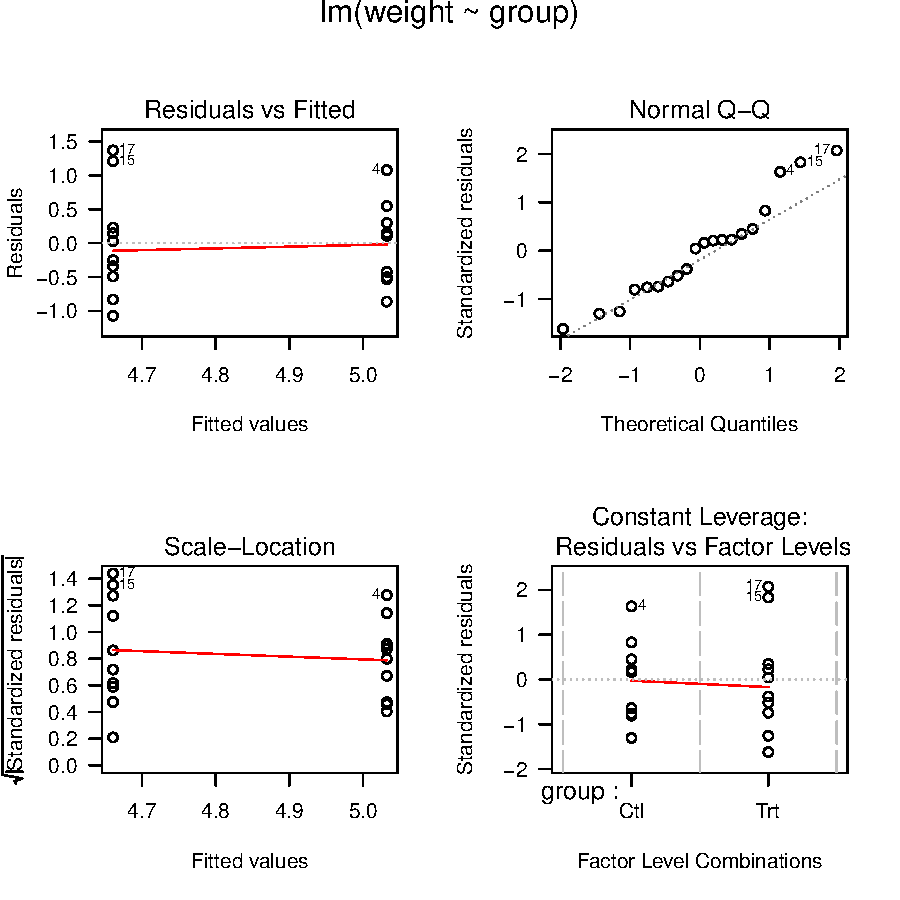
\includegraphics{sweave_example-summary_plot}
\end{center}
\caption{This is a summary of the linear regression.}
\label{fig:summarylm}
\end{figure}
\setkeys{Gin}{width=\textwidth}

\section*{Problem 5}
The last problem asked me to write a function to do $$\sqrt{b^2 - 4ac}$$.

\begin{Schunk}
\begin{Sinput}
> myfun = function(a,b,c){return(sqrt(b^2-4*a*c))}
> myfun(1,3,1)
\end{Sinput}
\begin{Soutput}
[1] 2.236068
\end{Soutput}
\end{Schunk}

\section*{Problem 6}

This problem asked me to write out a matrix equation $\mathbf{A}\mathbf{B}$ with $\mathbf{A}$ as a $3 \times 2$ matrix and $\mathbf{B}$ as a $2 \times 2$ matrix.  I chose this equation:
$$
\mathbf{A}\mathbf{B}=
\begin{bmatrix} 1 & 4\\ 2 & 5 \\ 3 & 6\end{bmatrix}
\begin{bmatrix} 3 & 0 \\ 0 & 3 \end{bmatrix}
$$
Here's my R code:

\begin{Schunk}
\begin{Sinput}
> A=matrix(1:6,3,2)
> B=diag(3,2)
> A%*%B
\end{Sinput}
\begin{Soutput}
     [,1] [,2]
[1,]    3   12
[2,]    6   15
[3,]    9   18
\end{Soutput}
\end{Schunk}


\end{document}
